\documentclass{article}

\usepackage[a4paper, hmargin={20mm, 20mm}, vmargin={25mm, 30mm}]{geometry}
\usepackage[utf8]{inputenc}
\usepackage[english, main=portuguese]{babel}

\usepackage[hidelinks]{hyperref}
\usepackage{bookmark}
\usepackage{cancel}
\usepackage{comment}

\usepackage{array}
\usepackage{indentfirst}
\usepackage{multicol}
\usepackage{subfiles}

\usepackage{amsmath}
\usepackage{amssymb}
\usepackage{systeme}
\usepackage{float}
\usepackage{enumitem}
\restylefloat{table}

\usepackage{graphicx}
\graphicspath{ {./IMAGENS/} }

% Pacote para a definição de novas cores
\usepackage{xcolor}
% Definindo novas cores
\definecolor{darkgreen}{rgb}{0.0, 0.42, 0.24}
\definecolor{darkpurple}{rgb}{0.74, 0.2, 0.64}
\definecolor{darkblue}{rgb}{0.0, 0.28, 0.67}

% Configurando layout para mostrar codigos Java
\usepackage{listings}


\newcommand{\myStyle}{
\lstset{
    language=Octave,                            % the language of the code
    basicstyle=\ttfamily\small,               % the size of the fonts that are used for the code
    keywordstyle=\color{darkpurple}\bfseries, %
    stringstyle=\color{darkblue},             %
    commentstyle=\color{darkgreen},           %
    morecomment=[s][\color{blue}]{/**}{*/},   %
    extendedchars=true,                       %
    showtabs=false,                           % show tabs within strings adding particular underscores
    showspaces=false,                         % show spaces adding particular underscores
    showstringspaces=false,                   % underline spaces within strings
    numbers=left,                             % where to put the line-numbers
    numberstyle=\tiny\color{gray},            % the style that is used for the line-numbers
    stepnumber=1,                             % the step between two line-numbers. If it's 1, each line will be numbered
    numbersep=5pt,                            % how far the line-numbers are from the code
    frame=single,                             % adds a frame around the code
    rulecolor=\color{black},                  % if not set, the frame-color may be changed on line-breaks within not-black text
    breaklines=true,                          % sets automatic line breaking
    backgroundcolor=\color{white},            % choose the background color
    breakatwhitespace=true,                   % sets if automatic breaks should only happen at whitespace
    breakautoindent=false,                    %
    captionpos=b,                             % sets the caption-position to bottom
    xleftmargin=0pt,                          %
    tabsize=2,                                % sets default tabsize to 2 spaces
}}

\title{MS211 - Cálculo Numérico}
\author{Guilherme Nunes Trofino\\217276}
\date{\today}

\begin{document}
    \maketitle
\newpage

\section{Questão}
    \subsection{Modelagem}
        \paragraph{Teoria}Sabe-se que a quantidade de poluentes a uma certa altura $x$ do fundo de um corpo d'água de altura $h$ pode ser descrito de acordo com a seguinte equação de \textit{Problema de Valor de Contorno}:
            \begin{equation}
                \boxed{f(x) = - \alpha\cdot c''(x) + \nu\cdot c'(x) + \mu\cdot c(x)}\label{eq:1}
            \end{equation}
            \begin{equation}
                \boxed{c(0) = 0 \hspace{5mm} c'(H) = 0}\label{eq:2}
            \end{equation}
        Onde:
            \begin{enumerate}[noitemsep]
                \item $\alpha$: Representa a \textbf{Difusibilidade} desse poluente na água;
                \item $\nu$: Representa a \textbf{Velocidade} e direção da densidade de partículas;
                    \begin{enumerate}[noitemsep]
                        \item $\nu > 0$, deslocamento das partículas para cima;
                        \item $\nu < 0$, deslocamento das partículas para baixo;
                    \end{enumerate}
                        \item $\mu$: Representa o \textbf{Decaimento} desse poluente na água
            \end{enumerate}
        Considera-se que poluentes vem apenas das chuvas e, portanto, sua entrada no sistema ocorre apenas pela superfície d'água. Este comportamento pode ser descrito como segue:
            \begin{equation}
                \boxed{
                    f(x) = \begin{cases}
                        k, & x = H\\
                        0, & x \neq H
                    \end{cases}\label{eq:3}
                }
            \end{equation}

        \paragraph{Notações}Adota-se as seguintes notações ao longo dos cálculos por simplicidade:
            \begin{enumerate}[noitemsep]
                \item $c_{i}$ para representar $c(x_{i})$;
                \item $c'_{i}$ para representar $c'(x_{i})$;
                \item $c''_{i}$ para representar $c''(x_{i})$;
            \end{enumerate}
        Em seguida utiliza-se as seguintes expressões para as derivadas de primeira e segunda ordem, respectivamente representadas, para modificar a primeira formulação do problema, apresentado em \eqref{eq:1}:
            \[c'_{i} = \frac{c_{i+1} - c_{i-1}}{2\Delta x}\]
            \[c''_{i} = \frac{c_{i-1} - 2c_{i} + c_{i+1}}{\Delta x^{2}}\]
            \[f_{i} = - \alpha\cdot\left(\frac{c_{i-1} - 2c_{i} + c_{i+1}}{\Delta x^{2}}\right) + \nu\cdot\left(\frac{c_{i+1} - c_{i-1}}{2\Delta x}\right) + \mu\cdot c_{1}\]

        \paragraph{Reformulação}Reordenando as variavéis utilizadas na última equação tem-se a relação abaixo, base da solução numérica: 
            \begin{equation}
                \boxed{f_{i} = \left(-\frac{\alpha}{\Delta x^{2}} - \frac{\nu}{2\Delta x}\right) c_{i-1} + \left(\frac{2\alpha}{\Delta x^{2}} + \mu\right) c_{i} + \left( - \frac{\alpha}{\Delta x^{2}} + \frac{\nu}{2\Delta x}\right) c_{i+1}}\label{eq:4}
            \end{equation}
        Nota-se que a expressão será válida $\forall x_{i}$ e que $\Delta x = \frac{H}{n}$ será obtido dividindo a altura do corpo d'água pela quantidade de subintervalos a serem avaliados. Haverá portanto $n$ incógnitas, $c_1, c_2, \dots, c_n$ a serem avaliadas, pois como $c(0) = c(x_0)$ sabe-se que $c_0 = 0$ e, portanto, já conhecida.

        \paragraph{Considerações}A equação \eqref{eq:4} estará definida para as $n - 1$ primeiras linhas do sistema, resultando em vetor de variáveis $\vec{c} = [c_1, c_2, \dots, c_{n-1}, c_{n}]$. Analisando cada parcela dos termos das equações temos, considerando a condição \eqref{eq:3}:
            \begin{enumerate}[noitemsep]
                \item Quando $i = 1$:
                    \[\cancelto{0}{f_{1}} = \left(-\frac{\alpha}{\Delta x^{2}} - \frac{\nu}{2\Delta x}\right) \cancelto{0}{c_{0}} + \left(\frac{2\alpha}{\Delta x^{2}} + \mu\right) c_{1} + \left( - \frac{\alpha}{\Delta x^{2}} + \frac{\nu}{2\Delta x}\right) c_{2}\]
                \item Quando $i = 2, 3, \dots, n-1$:
                    \[\cancelto{0}{f_{i}} = \left(-\frac{\alpha}{\Delta x^{2}} - \frac{\nu}{2\Delta x}\right) c_{i-1} + \left(\frac{2\alpha}{\Delta x^{2}} + \mu\right) c_{i} + \left( - \frac{\alpha}{\Delta x^{2}} + \frac{\nu}{2\Delta x}\right) c_{i+1}\]
                \item Quando $i = n$:
                    \[f_{n} = \left(-\frac{\alpha}{\Delta x^{2}} - \frac{\nu}{2\Delta x}\right) c_{n-1} + \left(\frac{2\alpha}{\Delta x^{2}} + \mu\right) c_{n} + \left( - \frac{\alpha}{\Delta x^{2}} + \frac{\nu}{2\Delta x}\right) c_{n+1}\]
            \end{enumerate}
        Nota-se, a princípio, que não existe $c_{n+1}$, entretanto, sabe-se pela condição de contorno, que $c'(H) = 0$ e, aplicando esta informação na aproximação utilizada para a derivada de primeira ordem, obtem-se:
            \[c'_{n} = \frac{c_{n+1} - c_{n-1}}{2\Delta x} \rightarrow 0 = \frac{c_{n+1} - c_{n-1}}{2\Delta x} \rightarrow \boxed{c_{n+1} = c_{n-1}}\]
        Assim:
            \begin{enumerate}[noitemsep]
                \item Quando $i = n$:
                    \[f_{n} = \left(-\frac{2\alpha}{\Delta x^{2}} - \frac{\nu}{2\Delta x}\right) c_{n-1} + \left(\frac{2\alpha}{\Delta x^{2}} + \mu\right) c_{n}\]
            \end{enumerate}

        \paragraph{Sistema}Desta maneira pode-se representar, tomando as considerações apresentadas acima, um sistema linear, onde $n$ representa a quantidade de subintervalos:
            \[
                A = -\alpha-\nu\frac{\Delta x}{2} \hspace{5mm}
                B = +2\alpha+\mu\Delta x^2 \hspace{5mm}
                C = -\alpha+\nu\frac{\Delta x}{2} \hspace{5mm}
                D = -2\alpha \hspace{5mm}
                \Delta x = \frac{H}{n}
            \]
            \begin{equation}
                \boxed{
                    \underbrace{\begin{bmatrix}
                        B_{1} & C_{1} &        &         &         &   &\\
                        A_{2} & B_{2} & C_{2}  &         &         &   &\\
                              & A_{3} & B_{3}  & C_{3}   &         &   &\\
                              &       & \ddots & \ddots  & \ddots  &   &\\
                              &       &        & A_{n-2} & B_{n-2} & C_{n-2} &\\
                              &       &        &         & A_{n-1} & B_{n-1} & C_{n-1}\\
                              &       &        &         &         & D_{n}   & B_{n}\\
                    \end{bmatrix}}_{n \times n} \times
                    \underbrace{\begin{bmatrix}
                        c_{1}\\
                        c_{2}\\
                        c_{3}\\
                        \vdots\\
                        c_{n-2}\\
                        c_{n-1}\\
                        c_{n}\\
                    \end{bmatrix}}_{n \times 1} = 
                    \underbrace{\begin{bmatrix}
                        0\\
                        0\\
                        0\\
                        \vdots\\
                        0\\
                        0\\
                        f\Delta x^2\\
                    \end{bmatrix}}_{n \times 1}
                }
            \end{equation}

    \subsection{Desenvolvimento}
        \paragraph{Problema}Notou-se que a qualidade da água na lagoa do parque Ábaco pode ser descrita de acordo com seguinte PVC:
            \[
                \left\{
                \begin{array}{c l}
                    0.025 & = - \underbrace{(1 - 0.09(5 - x))}_{\alpha}\cdot c''(x) + \underbrace{- (0.2 - 0.01(5 - x))}_{\nu < 0}\cdot c'(x) + \underbrace{0.05}_{\mu}\cdot c(x)\\
                    c(0)  & = 0\\
                    c'(5) & = 0
                \end{array}
                \right.
            \]
        Onde $c(x)$ representa a quantidade de poluente presente na água a uma certa profundidade $x \in [0, 5]$ do lago. As condições de contorno para este problema são respectivamente:
            \begin{enumerate}[noitemsep]
                \item Não há poluentes no fundo do lago: $c (0) = 0$;
                \item Não há evaporação dos polentes: $c'(5) = 0$;
            \end{enumerate}

        \paragraph{Observação}Nota-se que, diferentemente do desenvolvimento apresentado, este problema possui um valor constante, $f(x) = 0.025$, assim o sistema elaborado será ligeiramente distinto.

    \subsection{Respostas}
        \paragraph{Questão 1.}Sistema Geral de Equações obtido pelo Método de Diferenças Finitas:
            \[
                \underbrace{\begin{bmatrix}
                    B_{1} & C_{1}  &         &         & \\
                    A_{2} & B_{2}  & C_{2}   &         & \\
                          & \ddots & \ddots  & \ddots  & \\
                          &        & A_{n-1} & B_{n-1} & C_{n-1}\\
                          &        &         & D_{n}   & B_{n}\\
                \end{bmatrix}}_{n \times n} \times
                \underbrace{\begin{bmatrix}
                    c_{1}\\
                    c_{2}\\
                    \vdots\\
                    c_{n-1}\\
                    c_{n}\\
                \end{bmatrix}}_{n \times 1} = 
                \underbrace{\begin{bmatrix}
                    f\Delta x^2\\
                    f\Delta x^2\\
                    \vdots\\
                    f\Delta x^2\\
                    f\Delta x^2\\
                \end{bmatrix}}_{n \times 1}
            \]
        Onde:
            \[
                \left\{
                    \begin{array}{c l}
                        A_{i}    & = -1 + 0.09(5 - x_{i}) + (0.2 - 0.01(5-x_{i}))\frac{\Delta x}{2}\\
                        B_{i}    & = +2 - 0.18(5 - x_{i}) + 0.05\Delta x^2\\
                        C_{i}    & = -1 + 0.09(5 - x_{i}) - (0.2 - 0.01(5-x_{i}))\frac{\Delta x}{2}\\
                        D_{i}    & = +2 - 0.18(5 - x_{i})\\
                        f        & = 0.025
                    \end{array}
                \right.
            \]

        \paragraph{Questão 2.}Solução Numérica representada Graficamente:
            \begin{figure}[h]
                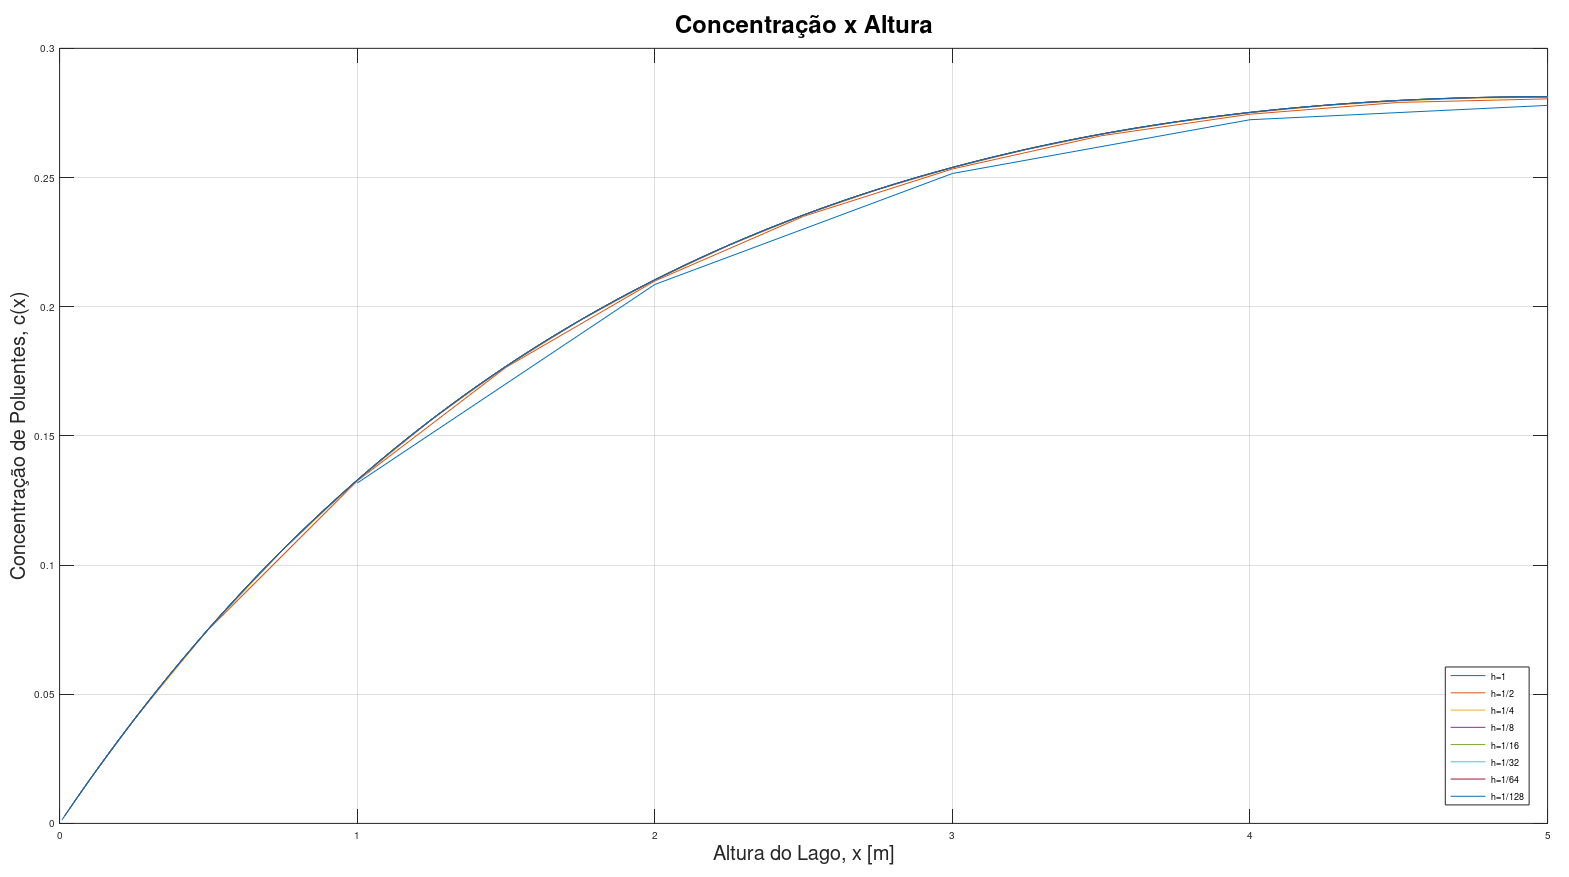
\includegraphics[width = 10cm]{grafico1.png}
                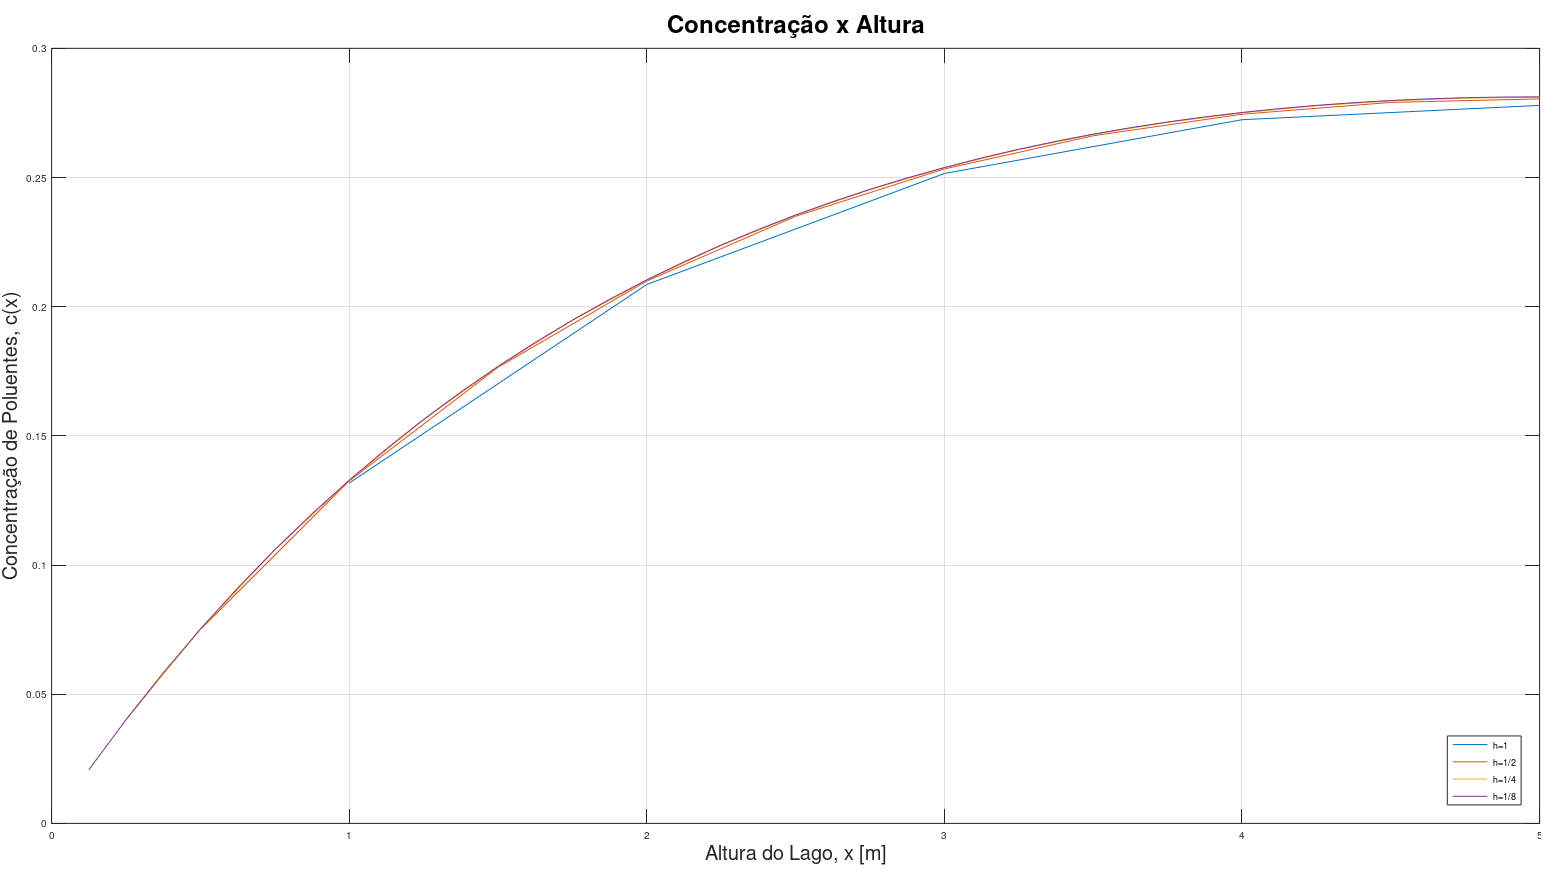
\includegraphics[width = 10cm]{grafico2.png}
                \centering
            \end{figure}

        \paragraph{Questão 3.}Nota-se que a partir $h = \frac{1}{8}$ não ouve mais mudanças significativas na solução como pode ser observado comparando os gráficos. As condições iniciais do problema aparentam estarem satisfeitas, visto que $c(0) = 0$, partida da origem, e $c'(5) = 0$, curva aproximadamente horizontal.
\newpage

    \subsection{Códigos}
\begin{scriptsize}
    \myStyle
    \begin{lstlisting}
%====================================================================================
function [X, C] = CriaSistemaLinear(A, V, U, f, H, dx)
    %================================================================================
    %Recebe Funcoes: A, V, U e f
    %Recebe Constantes: H e h
    %Retorna um Vetor X das Alturas e um Vetor C da Qntd. de Poluentes
    %================================================================================  
    n = H/dx;              %Qtde Intervalos
    M = zeros(n, n);       %Inicializa a Matriz Base
    N = f*ones(n, 1)*dx^2; %Inicializa o Vetor Base

    X = linspace(dx, H, n); %Inicializa o Vetor de Intervalos

    for(i = 1: n)
        if(i != 1)
            M(i, i-1) = -A(X(i), H) -V(X(i), H)*dx/2; %Diagonal Inferior
        endif

        M(i, i) = 2*A(X(i), H) + U*dx^2; %Diagonal Principal
    
        if(i != n)
            M(i, i+1) = -A(X(i), H) +V(X(i), H)*dx/2; %Diagonal Superior
        endif 
    endfor
    
    M(n, n-1) = -2*A(X(n), H); %Modifica a Entrada (n, n-1)
    C = M\N;              %Soluciona o Sistema Linear
endfunction

%====================================================================================
%Declaracao das Funcoes e Variaveis
f = 0.025; %Funcao Constante
H = 5;     %Altura do Lago

A = @(x, H)  (1 - 0.09*(H - x));   %alpha
V = @(x, H) -(0.2 - 0.01*(H - x)); %nu
U = 0.05;                          %mu

%CriaSistemaLinear recebe alpha/nu/mu/f(x)/altura/intervalo
[X1, C1] = CriaSistemaLinear(A, V, U, f, H, 1    ); %Solucao h=1
[X2, C2] = CriaSistemaLinear(A, V, U, f, H, 1/2  ); %Solucao h=1/2
[X3, C3] = CriaSistemaLinear(A, V, U, f, H, 1/4  ); %Solucao h=1/4
[X4, C4] = CriaSistemaLinear(A, V, U, f, H, 1/8  ); %Solucao h=1/8
[X5, C5] = CriaSistemaLinear(A, V, U, f, H, 1/16 ); %Solucao h=1/16
[X6, C6] = CriaSistemaLinear(A, V, U, f, H, 1/32 ); %Solucao h=1/32
[X7, C7] = CriaSistemaLinear(A, V, U, f, H, 1/64 ); %Solucao h=1/64
[X8, C8] = CriaSistemaLinear(A, V, U, f, H, 1/128); %Solucao h=1/128


%Criacao do Grafico
LW = 1; FS = 20;
plot(X1,C1,'linewidth',LW,X2,C2,'linewidth',LW,
        X3,C3,'linewidth',LW,X4,C4,'linewidth',LW,
        X5,C5,'linewidth',LW,X6,C6,'linewidth',LW,
        X7,C7,'linewidth',LW,X8,C8,'linewidth',LW); grid;
title("Concentracao x Altura","fontsize",FS+4);
xlabel("Altura do Lago, x [m]","fontsize",FS);
ylabel("Concentracao de Poluentes, c(x)","fontsize",FS);
legend("h=1","h=1/2","h=1/4","h=1/8","h=1/16","h=1/32","h=1/64","h=1/128", 
        "location", "southeast"); axis([0 H]);
    \end{lstlisting}
\end{scriptsize}
\newpage

\section{Questão}
    \subsection{Modelagem}
        \paragraph{Teoria}Sabe-se que, a partir de uma tabela de dados, pode-se obter uma função $\varphi$ que interpola, isto é, relacionara todos os pontos fornecidos como descrito:
            \[
                \begin{tabular}{c | c c c}
                    x & $x_{1}$ & \dots & $x_{n}$\\ \hline
                    y & $y_{1}$ & \dots & $y_{n}$
                \end{tabular}
            \]
            \begin{equation}
                \boxed{\varphi(x_{k}) = y_{k}, \hspace{2.5mm} \forall k = 1, \dots, n}
            \end{equation}
        Há diferentes métodos para se estimar a Interpolação Linear para um conjunto de dados, dos quais são notáveis:
            \begin{enumerate}[noitemsep]
                \item Forma de Vandermonde;
                \item Forma de Lagrande;
                \item Forma de Newton;
            \end{enumerate}
        Utiliza-se a Forma de Newton por sua simplicidade e reduzido custo computacional de execução quando comparado com o Forma de Lagrange, por exemplo, que apesar de direta é computacionalmente custosa.

        \paragraph{Forma de Newton}Nesta abordagem o sistema linear resultante será triangular inferior descrito pelas seguintes funções base:
            \[
                \begin{array}{c l}
                    N_{0} & = 1\\
                    N_{1} & = x - x_{0}\\
                    N_{2} & = (x - x_{0})(x - x_{1})\\
                    \vdots&\\
                    N_{n} & = (x - x_{0})(x - x_{1})\cdots(x - x_{n-2})(x - x_{n-1})\\
                \end{array}
            \]
        Consequentemente os coeficientes do polinômio interpolador $\varphi$ podem ser obtidos solucionando o sistemas linear apresentado anteriormente:
            \[\boxed{\varphi_{n}(x) = \alpha_{0} + \alpha_{1}(x - x_{0}) + \cdots + \alpha_{n}(x - x_{0})(x - x_{1})\cdots(x -x_{n-1})}\]

        \paragraph{Operador Diferenças Dividas}Alternativamente os coeficientes do polinômio interpolador podem ser calculados utilizando \textbf{Diferenças Dividas} denotadas em sequência:
            \[\boxed{\alpha_{k} = f[x_{0}, x_{1}, \dots, x_{k}], \hspace{2.5mm} \forall k = 0, 1, \dots, n}\]

        \paragraph{Erro da Interpolação}Nas considerações apresentadas o erro poderá ser estimado pela seguinte expressão:
            \[\boxed{\epsilon_{n}(x) \approx \max_{x\in [x_{0}, x_{n}]}|f^{(n+1)}(x)|\prod_{k=0}^{n}|(x - x_{k})|}\]

        \paragraph{Fenômeno de Runge}Nota-se que em interpolações realizadas em intervalos igualmente espaçadas há oscilação nas bordas de um intervalo em polinomios de grau elevado. Isso implica que a medida que o grau do polinômio interpolador aumenta cresce também o erro associado.

    \subsection{Desenvolvimento}
        \paragraph{Problema}Notou-se que o registro do número de casos graves de COVID-19 ao longo de 2 meses na Sobolévia apresentou falha em 15/11 como mostrado:
            \[
                \begin{tabular}{c c}
                    Data  & Casos\\ \hline
                    29/11 & 2899 \\
                    22/11 & 3118 \\
                    15/11 & ???  \\
                    08/11 & 2821 \\
                    01/11 & 2294 \\
                    25/10 & 2261 \\
                    18/10 & 2219 \\
                    10/10 & 2347 \\
                    04/10 & 2546
                \end{tabular}
            \]
        Afim de estimar, por meio da Interpolação Linear, o número de casos em 15/11 será necessário, primeiramente, modificar esta tabela para que sejam considerados apenas os dias das datas fornecidas, tomando 04/10 como dia 0. Em seguida, exclui-se o dado a ser calculado, modificando também a nomenclatura das colunas.
            \[
                \begin{tabular}{c c}
                    Data  & Casos\\ \hline
                    29/11 & 2899\\
                    22/11 & 3118\\
                    15/11 & ??? \\
                    08/11 & 2821\\
                    01/11 & 2294\\
                    25/10 & 2261\\
                    18/10 & 2219\\
                    10/10 & 2347\\
                    04/10 & 2546
                \end{tabular} \hspace{2.5mm} \rightarrow \hspace{2.5mm}
                \begin{tabular}{c c}
                    Dia  & Casos\\ \hline
                    54   & 2899\\
                    47   & 3118\\
                    44   & ??? \\
                    33   & 2821\\
                    28   & 2294\\
                    21   & 2261\\
                    14   & 2219\\
                    6    & 2347\\
                    0    & 2546
                \end{tabular} \hspace{2.5mm} \rightarrow \hspace{2.5mm}
                \begin{tabular}{c c}
                    X  & Y\\ \hline
                    54 & 2899\\
                    47 & 3118\\
                       &     \\
                    33 & 2821\\
                    28 & 2294\\
                    21 & 2261\\
                    14 & 2219\\
                    6  & 2347\\
                    0  & 2546
                \end{tabular}
            \]

        \paragraph{Observação}Caso fosse considerado 04/10 como dia 4 os resultados seriam ligeiramente distintos e, portanto deve-se atentar a escolha de datas.

    \subsection{Respostas}
        \paragraph{Questão 1.}Levando em consideração os conceitos empregados no \textbf{Fenômeno de Runge}, apesar do problema do problema não possuir intervalos igualmente espaçados, espera-se que quanto maior o grau do polinômio mais sucetível a erro a aproximação estará. Assim escolheu-se um Polinômio de Grau 4 para realização da interpolação, utilizando o seguinte conjunto de dados:
            \[
                \begin{tabular}{c c}
                    X  & Y\\ \hline
                    54 & 2899\\
                    47 & 3118\\
                       & \\
                    33 & 2821\\
                    28 & 2294\\
                \end{tabular}
            \]
        Escolhendo este conjunto de dados para um polinômio interpolador estima-se aproximadamente 3161.4 casos graves de COVID-19 com erro relativo de 150.33 casos para o dia 15/11.
\newpage

    \subsection{Código}
\begin{scriptsize}
    \myStyle
    \begin{lstlisting}
%====================================================================================
function [T] = CoeficientesNewton (X, Y)
    %================================================================================
    %Recebe Vetores: X e Y
    %Retorna um Vetor C com os Coeficientes de Newton do Conjunto
    %================================================================================
    nPontos = length(X);         %Qtde de Dados
    T = zeros(nPontos, nPontos); %Matriz das Diferencas Dividas
    T(:,1) = Y;                  %Inicializa a Primeira Coluna
    
    for(j = 2:nPontos)
        for(i = 1:(nPontos-j+1))
            
            T(i,j) = (T(i+1,j-1) - T(i,j-1))/(X(j+i-1) - X(i)); %Calculo das Entradas
            
        endfor
    endfor  
endfunction

%====================================================================================
function y = CalculoInterpolacao(A, X, T)
    %================================================================================
    %Recebe o Valor A, o Vetor X e a Matrix T
    %Retorna um Valor y da Interpolacao
    %================================================================================
  C = T(1,:); %Obtem os Coeficientes de Interpolacao
  y = C(1);   %Valor Base da Interpolacao
  
  for(i = 2:length(C)) 
    produto = C(i); %Inicializa o Produto
    
    for(j = 1:i-1)
      produto = produto*(A - X(j)); %Realiza o Produtorio
    endfor
    
    y = y + produto; %Realiza o Somatorio
  endfor
endfunction

%====================================================================================
function e = ErroInterpolacao(A, X, T)
    %================================================================================
    %Recebe Vetores: X e Y
    %Retorna um Vetor C com os Coeficientes de Newton do Conjunto
    %================================================================================
  e = 1; %Inicializa o Erro
    
  for(i = 1:length(X)) 
    e = abs(e*(A - X(i))); %Realiza o Produtorio
  endfor
  
  maxF = 0; %Inicializa o Maximo
  for(i = 1:(size(T)(1)))
    if(abs(T(i,(size(T)(2)))) > maxF)
      maxF = abs(T(i,(size(T)(2)))); %Modifica o Maximo
    endif
  endfor
  
  e = e*maxF; %Retorna o Erro da Interpolacao
endfunction


%====================================================================================
%Declaracao das Colunas de Constantes
X = [0 6 14 21 28 33 47 54]';                   %Contagem em Dias
Y = [2546 2347 2219 2261 2294 2821 3118 2899]'; %Numero de Casos

T = CoeficientesNewton(X, Y); %Obtencao dos Coeficientes de Newton

S = 5;  %Start 
E = 8;  %End
A = 44; %Dia 44

y = CalculoInterpolacao(A, X(S:E), T(S:end,1:E-S+1)) %Retorna Numero de Casos
E = ErroInterpolacao(A, X(S:E), T(:,1:E-S+2))        %Retorna Erro da Interpolacao
    \end{lstlisting}
\end{scriptsize}

\end{document}